\pgfdeclareplotmark{cross} {
\pgfpathmoveto{\pgfpoint{-0.3\pgfplotmarksize}{\pgfplotmarksize}}
\pgfpathlineto{\pgfpoint{+0.3\pgfplotmarksize}{\pgfplotmarksize}}
\pgfpathlineto{\pgfpoint{+0.3\pgfplotmarksize}{0.3\pgfplotmarksize}}
\pgfpathlineto{\pgfpoint{+1\pgfplotmarksize}{0.3\pgfplotmarksize}}
\pgfpathlineto{\pgfpoint{+1\pgfplotmarksize}{-0.3\pgfplotmarksize}}
\pgfpathlineto{\pgfpoint{+0.3\pgfplotmarksize}{-0.3\pgfplotmarksize}}
\pgfpathlineto{\pgfpoint{+0.3\pgfplotmarksize}{-1.\pgfplotmarksize}}
\pgfpathlineto{\pgfpoint{-0.3\pgfplotmarksize}{-1.\pgfplotmarksize}}
\pgfpathlineto{\pgfpoint{-0.3\pgfplotmarksize}{-0.3\pgfplotmarksize}}
\pgfpathlineto{\pgfpoint{-1.\pgfplotmarksize}{-0.3\pgfplotmarksize}}
\pgfpathlineto{\pgfpoint{-1.\pgfplotmarksize}{0.3\pgfplotmarksize}}
\pgfpathlineto{\pgfpoint{-0.3\pgfplotmarksize}{0.3\pgfplotmarksize}}
\pgfpathclose
\pgfusepathqstroke
}
\pgfdeclareplotmark{cross*} {
\pgfpathmoveto{\pgfpoint{-0.3\pgfplotmarksize}{\pgfplotmarksize}}
\pgfpathlineto{\pgfpoint{+0.3\pgfplotmarksize}{\pgfplotmarksize}}
\pgfpathlineto{\pgfpoint{+0.3\pgfplotmarksize}{0.3\pgfplotmarksize}}
\pgfpathlineto{\pgfpoint{+1\pgfplotmarksize}{0.3\pgfplotmarksize}}
\pgfpathlineto{\pgfpoint{+1\pgfplotmarksize}{-0.3\pgfplotmarksize}}
\pgfpathlineto{\pgfpoint{+0.3\pgfplotmarksize}{-0.3\pgfplotmarksize}}
\pgfpathlineto{\pgfpoint{+0.3\pgfplotmarksize}{-1.\pgfplotmarksize}}
\pgfpathlineto{\pgfpoint{-0.3\pgfplotmarksize}{-1.\pgfplotmarksize}}
\pgfpathlineto{\pgfpoint{-0.3\pgfplotmarksize}{-0.3\pgfplotmarksize}}
\pgfpathlineto{\pgfpoint{-1.\pgfplotmarksize}{-0.3\pgfplotmarksize}}
\pgfpathlineto{\pgfpoint{-1.\pgfplotmarksize}{0.3\pgfplotmarksize}}
\pgfpathlineto{\pgfpoint{-0.3\pgfplotmarksize}{0.3\pgfplotmarksize}}
\pgfpathclose
\pgfusepathqfillstroke
}
\pgfdeclareplotmark{newstar} {
\pgfpathmoveto{\pgfqpoint{0pt}{\pgfplotmarksize}}
\pgfpathlineto{\pgfqpointpolar{44}{0.5\pgfplotmarksize}}
\pgfpathlineto{\pgfqpointpolar{18}{\pgfplotmarksize}}
\pgfpathlineto{\pgfqpointpolar{-20}{0.5\pgfplotmarksize}}
\pgfpathlineto{\pgfqpointpolar{-54}{\pgfplotmarksize}}
\pgfpathlineto{\pgfqpointpolar{-90}{0.5\pgfplotmarksize}}
\pgfpathlineto{\pgfqpointpolar{234}{\pgfplotmarksize}}
\pgfpathlineto{\pgfqpointpolar{198}{0.5\pgfplotmarksize}}
\pgfpathlineto{\pgfqpointpolar{162}{\pgfplotmarksize}}
\pgfpathlineto{\pgfqpointpolar{134}{0.5\pgfplotmarksize}}
\pgfpathclose
\pgfusepathqstroke
}
\pgfdeclareplotmark{newstar*} {
\pgfpathmoveto{\pgfqpoint{0pt}{\pgfplotmarksize}}
\pgfpathlineto{\pgfqpointpolar{44}{0.5\pgfplotmarksize}}
\pgfpathlineto{\pgfqpointpolar{18}{\pgfplotmarksize}}
\pgfpathlineto{\pgfqpointpolar{-20}{0.5\pgfplotmarksize}}
\pgfpathlineto{\pgfqpointpolar{-54}{\pgfplotmarksize}}
\pgfpathlineto{\pgfqpointpolar{-90}{0.5\pgfplotmarksize}}
\pgfpathlineto{\pgfqpointpolar{234}{\pgfplotmarksize}}
\pgfpathlineto{\pgfqpointpolar{198}{0.5\pgfplotmarksize}}
\pgfpathlineto{\pgfqpointpolar{162}{\pgfplotmarksize}}
\pgfpathlineto{\pgfqpointpolar{134}{0.5\pgfplotmarksize}}
\pgfpathclose
\pgfusepathqfillstroke
}
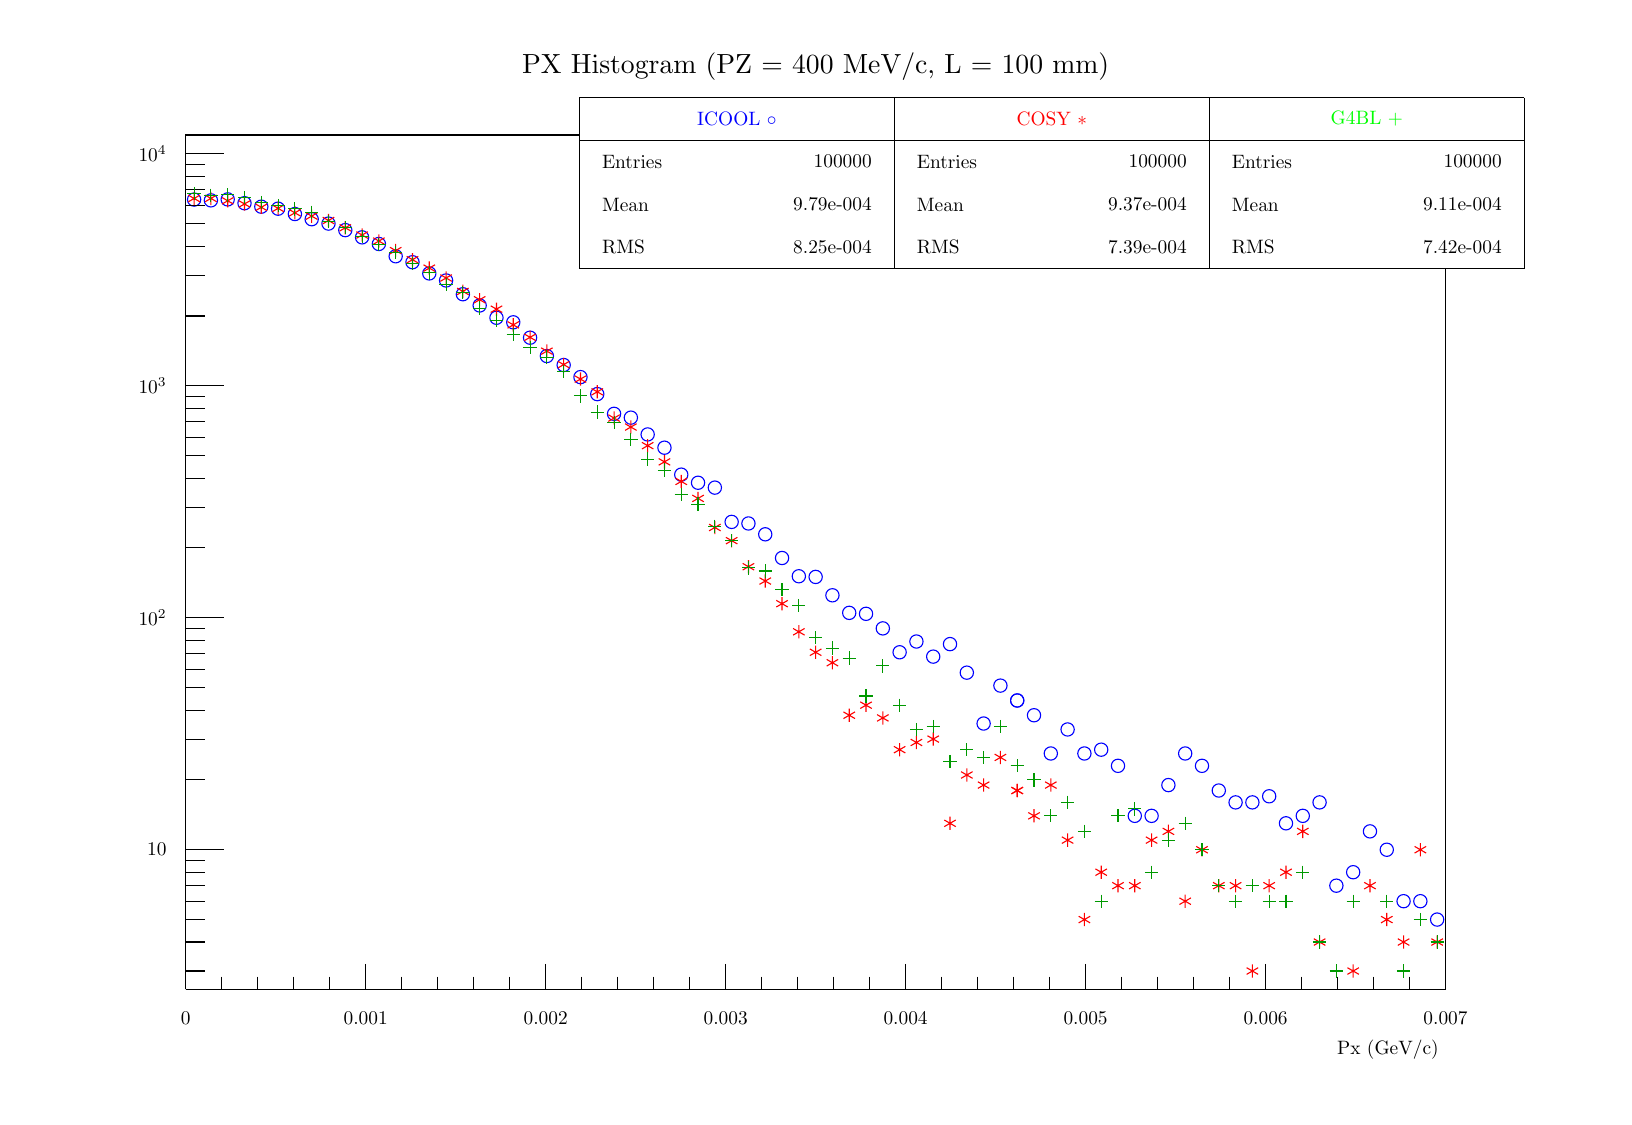
\begin{tikzpicture}
\definecolor{c}{rgb}{1,1,1};
\draw [color=c, fill=c] (0,0) rectangle (20,13.5632);
\draw [color=c, fill=c] (2,1.35632) rectangle (18,12.2069);
\definecolor{c}{rgb}{0,0,0};
\draw [c] (2,1.35632) -- (2,12.2069) -- (18,12.2069) -- (18,1.35632) -- (2,1.35632);
\definecolor{c}{rgb}{1,1,1};
\draw [color=c, fill=c] (2,1.35632) rectangle (18,12.2069);
\definecolor{c}{rgb}{0,0,0};
\draw [c] (2,1.35632) -- (2,12.2069) -- (18,12.2069) -- (18,1.35632) -- (2,1.35632);
\definecolor{c}{rgb}{0,0,1};
\foreach \P in
 {(2.10667,11.387),(2.32,11.3771),(2.53333,11.3892),(2.74667,11.3409),(2.96,11.2965),(3.17333,11.2714),(3.38667,11.2034),(3.6,11.1376),(3.81333,11.0821),(4.02667,10.9991),(4.24,10.9073),(4.45333,10.8231),(4.66667,10.6671),(4.88,10.5914),(5.09333,10.4
49),(5.30667,10.3596),(5.52,10.185),(5.73333,10.0422),(5.94667,9.88613),(6.16,9.82819),(6.37333,9.63278),(6.58667,9.40015),(6.8,9.28571),(7.01333,9.13215),(7.22667,8.9166),(7.44,8.66571),(7.65333,8.61749),(7.86667,8.40408),(8.08,8.2359),(8.29333,7.89
359),(8.50667,7.79067),(8.72,7.72891),(8.93333,7.29349),(9.14667,7.27358),(9.36,7.13599),(9.57333,6.83504),(9.78667,6.60319),(10,6.59469),(10.2133,6.36142),(10.4267,6.13835),(10.64,6.12611),(10.8533,5.94113),(11.0667,5.63774),(11.28,5.77434),(11.4933
,5.58251),(11.7067,5.74154),(11.92,5.379),(12.1333,4.73277),(12.3467,5.21444),(12.56,5.02555)}{\draw[mark options={color=c,fill=c},mark size=2.402402pt,mark=o] plot coordinates {\P};}
\foreach \P in
 {(12.56,5.02555),(12.7733,4.83799),(12.9867,4.35246),(13.2,4.65749),(13.4133,4.35246),(13.6267,4.40075),(13.84,4.1956),(14.0533,3.56046),(14.2667,3.56046),(14.48,3.95117),(14.6933,4.35246),(14.9067,4.1956),(15.12,3.88199),(15.3333,3.7313),(15.5467,3
.7313),(15.76,3.80886),(15.9733,3.46564),(16.1867,3.56046),(16.4,3.7313),(16.6133,2.67363),(16.8267,2.84447),(17.04,3.36323),(17.2533,3.12997),(17.4667,2.47641),(17.68,2.47641),(17.8933,2.24314)}{\draw[mark options={color=c,fill=c},mark
 size=2.402402pt,mark=o] plot coordinates {\P};}
\definecolor{c}{rgb}{1,1,1};
\draw [color=c, fill=c] (7,10.5115) rectangle (11,12.6816);
\definecolor{c}{rgb}{0,0,0};
\draw [c] (7,10.5115) -- (11,10.5115);
\draw [c] (11,10.5115) -- (11,12.6816);
\draw [c] (11,12.6816) -- (7,12.6816);
\draw [c] (7,12.6816) -- (7,10.5115);
\draw[color=blue](9,12.4103) node[scale=0.7, rotate=0]{ICOOL $\circ$};
\draw [c] (7,12.1391) -- (11,12.1391);
\draw [anchor= west] (7.2,11.8678) node[scale=0.6, rotate=0]{Entries };
\draw [anchor= east] (10.8,11.8678) node[scale=0.6, rotate=0]{ 100000};
\draw [anchor= west] (7.2,11.3253) node[scale=0.6, rotate=0]{Mean  };
\draw [anchor= east] (10.8,11.3253) node[scale=0.6, rotate=0]{ 9.79e-004};
\draw [anchor= west] (7.2,10.7828) node[scale=0.6, rotate=0]{RMS   };
\draw [anchor= east] (10.8,10.7828) node[scale=0.6, rotate=0]{ 8.25e-004};
\draw [c] (2,1.35632) -- (18,1.35632);
\draw [anchor= east] (18,0.596782) node[scale=0.7, rotate=0]{Px (GeV/c)};
\draw [c] (2,1.68184) -- (2,1.35632);
\draw [c] (2.45714,1.51908) -- (2.45714,1.35632);
\draw [c] (2.91429,1.51908) -- (2.91429,1.35632);
\draw [c] (3.37143,1.51908) -- (3.37143,1.35632);
\draw [c] (3.82857,1.51908) -- (3.82857,1.35632);
\draw [c] (4.28571,1.68184) -- (4.28571,1.35632);
\draw [c] (4.74286,1.51908) -- (4.74286,1.35632);
\draw [c] (5.2,1.51908) -- (5.2,1.35632);
\draw [c] (5.65714,1.51908) -- (5.65714,1.35632);
\draw [c] (6.11429,1.51908) -- (6.11429,1.35632);
\draw [c] (6.57143,1.68184) -- (6.57143,1.35632);
\draw [c] (7.02857,1.51908) -- (7.02857,1.35632);
\draw [c] (7.48571,1.51908) -- (7.48571,1.35632);
\draw [c] (7.94286,1.51908) -- (7.94286,1.35632);
\draw [c] (8.4,1.51908) -- (8.4,1.35632);
\draw [c] (8.85714,1.68184) -- (8.85714,1.35632);
\draw [c] (9.31429,1.51908) -- (9.31429,1.35632);
\draw [c] (9.77143,1.51908) -- (9.77143,1.35632);
\draw [c] (10.2286,1.51908) -- (10.2286,1.35632);
\draw [c] (10.6857,1.51908) -- (10.6857,1.35632);
\draw [c] (11.1429,1.68184) -- (11.1429,1.35632);
\draw [c] (11.6,1.51908) -- (11.6,1.35632);
\draw [c] (12.0571,1.51908) -- (12.0571,1.35632);
\draw [c] (12.5143,1.51908) -- (12.5143,1.35632);
\draw [c] (12.9714,1.51908) -- (12.9714,1.35632);
\draw [c] (13.4286,1.68184) -- (13.4286,1.35632);
\draw [c] (13.8857,1.51908) -- (13.8857,1.35632);
\draw [c] (14.3429,1.51908) -- (14.3429,1.35632);
\draw [c] (14.8,1.51908) -- (14.8,1.35632);
\draw [c] (15.2571,1.51908) -- (15.2571,1.35632);
\draw [c] (15.7143,1.68184) -- (15.7143,1.35632);
\draw [c] (16.1714,1.51908) -- (16.1714,1.35632);
\draw [c] (16.6286,1.51908) -- (16.6286,1.35632);
\draw [c] (17.0857,1.51908) -- (17.0857,1.35632);
\draw [c] (17.5429,1.51908) -- (17.5429,1.35632);
\draw [c] (18,1.68184) -- (18,1.35632);
\draw [c] (18,1.68184) -- (18,1.35632);
\draw [anchor=base] (2,0.908736) node[scale=0.7, rotate=0]{0};
\draw [anchor=base] (4.28571,0.908736) node[scale=0.7, rotate=0]{0.001};
\draw [anchor=base] (6.57143,0.908736) node[scale=0.7, rotate=0]{0.002};
\draw [anchor=base] (8.85714,0.908736) node[scale=0.7, rotate=0]{0.003};
\draw [anchor=base] (11.1429,0.908736) node[scale=0.7, rotate=0]{0.004};
\draw [anchor=base] (13.4286,0.908736) node[scale=0.7, rotate=0]{0.005};
\draw [anchor=base] (15.7143,0.908736) node[scale=0.7, rotate=0]{0.006};
\draw [anchor=base] (18,0.908736) node[scale=0.7, rotate=0]{0.007};
\draw [c] (2,1.35632) -- (2,12.2069);
\draw [c] (2.24,1.58958) -- (2,1.58958);
\draw [c] (2.24,1.95765) -- (2,1.95765);
\draw [c] (2.24,2.24314) -- (2,2.24314);
\draw [c] (2.24,2.47641) -- (2,2.47641);
\draw [c] (2.24,2.67363) -- (2,2.67363);
\draw [c] (2.24,2.84447) -- (2,2.84447);
\draw [c] (2.24,2.99517) -- (2,2.99517);
\draw [c] (2.48,3.12997) -- (2,3.12997);
\draw [anchor= east] (1.844,3.12997) node[scale=0.7, rotate=0]{10};
\draw [c] (2.24,4.01679) -- (2,4.01679);
\draw [c] (2.24,4.53555) -- (2,4.53555);
\draw [c] (2.24,4.90361) -- (2,4.90361);
\draw [c] (2.24,5.1891) -- (2,5.1891);
\draw [c] (2.24,5.42237) -- (2,5.42237);
\draw [c] (2.24,5.61959) -- (2,5.61959);
\draw [c] (2.24,5.79043) -- (2,5.79043);
\draw [c] (2.24,5.94113) -- (2,5.94113);
\draw [c] (2.48,6.07593) -- (2,6.07593);
\draw [anchor= east] (1.844,6.07593) node[scale=0.7, rotate=0]{$10^{2}$};
\draw [c] (2.24,6.96275) -- (2,6.96275);
\draw [c] (2.24,7.48151) -- (2,7.48151);
\draw [c] (2.24,7.84957) -- (2,7.84957);
\draw [c] (2.24,8.13507) -- (2,8.13507);
\draw [c] (2.24,8.36833) -- (2,8.36833);
\draw [c] (2.24,8.56556) -- (2,8.56556);
\draw [c] (2.24,8.7364) -- (2,8.7364);
\draw [c] (2.24,8.88709) -- (2,8.88709);
\draw [c] (2.48,9.02189) -- (2,9.02189);
\draw [anchor= east] (1.844,9.02189) node[scale=0.7, rotate=0]{$10^{3}$};
\draw [c] (2.24,9.90871) -- (2,9.90871);
\draw [c] (2.24,10.4275) -- (2,10.4275);
\draw [c] (2.24,10.7955) -- (2,10.7955);
\draw [c] (2.24,11.081) -- (2,11.081);
\draw [c] (2.24,11.3143) -- (2,11.3143);
\draw [c] (2.24,11.5115) -- (2,11.5115);
\draw [c] (2.24,11.6824) -- (2,11.6824);
\draw [c] (2.24,11.8331) -- (2,11.8331);
\draw [c] (2.48,11.9679) -- (2,11.9679);
\draw [anchor= east] (1.844,11.9679) node[scale=0.7, rotate=0]{$10^{4}$};
\definecolor{c}{rgb}{1,1,1};
\draw [color=c, fill=c] (7,10.5115) rectangle (11,12.6816);
\definecolor{c}{rgb}{0,0,0};
\draw [c] (7,10.5115) -- (11,10.5115);
\draw [c] (11,10.5115) -- (11,12.6816);
\draw [c] (11,12.6816) -- (7,12.6816);
\draw [c] (7,12.6816) -- (7,10.5115);
\draw[color=blue](9,12.4103) node[scale=0.7, rotate=0]{ICOOL $\circ$};
\draw [c] (7,12.1391) -- (11,12.1391);
\draw [anchor= west] (7.2,11.8678) node[scale=0.7, rotate=0]{Entries };
\draw [anchor= east] (10.8,11.8678) node[scale=0.7, rotate=0]{ 100000};
\draw [anchor= west] (7.2,11.3253) node[scale=0.7, rotate=0]{Mean  };
\draw [anchor= east] (10.8,11.3253) node[scale=0.7, rotate=0]{ 9.79e-004};
\draw [anchor= west] (7.2,10.7828) node[scale=0.7, rotate=0]{RMS   };
\draw [anchor= east] (10.8,10.7828) node[scale=0.7, rotate=0]{ 8.25e-004};
\draw (10,13.0816) node[scale=1, rotate=0]{PX Histogram (PZ = 400 MeV/c, L = 100 mm)};
\definecolor{c}{rgb}{1,0,0};
\foreach \P in
 {(2.10667,11.4009),(2.32,11.4017),(2.53333,11.3714),(2.74667,11.3312),(2.96,11.2889),(3.17333,11.2755),(3.38667,11.2187),(3.6,11.1769),(3.81333,11.1208),(4.02667,11.0285),(4.24,10.9368),(4.45333,10.8601),(4.66667,10.7393),(4.88,10.6236),(5.09333,10.
5168),(5.30667,10.3911),(5.52,10.221),(5.73333,10.115),(5.94667,9.99528),(6.16,9.79576),(6.37333,9.63753),(6.58667,9.46239),(6.8,9.2909),(7.01333,9.10726),(7.22667,8.94545),(7.44,8.61222),(7.65333,8.49801),(7.86667,8.26165),(8.08,8.0559),(8.29333,7.8
073),(8.50667,7.59177),(8.72,7.2224),(8.93333,7.05528),(9.14667,6.72436),(9.36,6.54246),(9.57333,6.25474),(9.78667,5.89776),(10,5.63774),(10.2133,5.50494),(10.4267,4.83799),(10.64,4.96604),(10.8533,4.80387),(11.0667,4.40075),(11.28,4.49217),(11.4933,
4.53555),(11.7067,3.46564),(11.92,4.07921),(12.1333,3.95117),(12.3467,4.30228),(12.56,3.88199)}{\draw[mark options={color=c,fill=c},mark size=2.402402pt,mark=asterisk] plot coordinates {\P};}
\foreach \P in
 {(12.56,3.88199),(12.7733,3.56046),(12.9867,3.95117),(13.2,3.25191),(13.4133,2.24314),(13.6267,2.84447),(13.84,2.67363),(14.0533,2.67363),(14.2667,3.25191),(14.48,3.36323),(14.6933,2.47641),(14.9067,3.12997),(15.12,2.67363),(15.3333,2.67363),(15.546
7,1.58959),(15.76,2.67363),(15.9733,2.84447),(16.1867,3.36323),(16.4,1.95765),(16.8267,1.58959),(17.04,2.67363),(17.2533,2.24314),(17.4667,1.95765),(17.68,3.12997),(17.8933,1.95765)}{\draw[mark options={color=c,fill=c},mark
 size=2.402402pt,mark=asterisk] plot coordinates {\P};}
\definecolor{c}{rgb}{1,1,1};
\draw [color=c, fill=c] (11,10.5115) rectangle (15,12.6816);
\definecolor{c}{rgb}{0,0,0};
\draw [c] (11,10.5115) -- (15,10.5115);
\draw [c] (15,10.5115) -- (15,12.6816);
\draw [c] (15,12.6816) -- (11,12.6816);
\draw [c] (11,12.6816) -- (11,10.5115);
\draw [color=red](13,12.4103) node[scale=0.7, rotate=0]{COSY $*$};
\draw [c] (11,12.1391) -- (15,12.1391);
\draw [anchor= west] (11.2,11.8678) node[scale=0.7, rotate=0]{Entries };
\draw [anchor= east] (14.8,11.8678) node[scale=0.7, rotate=0]{ 100000};
\draw [anchor= west] (11.2,11.3253) node[scale=0.7, rotate=0]{Mean  };
\draw [anchor= east] (14.8,11.3253) node[scale=0.7, rotate=0]{ 9.37e-004};
\draw [anchor= west] (11.2,10.7828) node[scale=0.7, rotate=0]{RMS   };
\draw [anchor= east] (14.8,10.7828) node[scale=0.7, rotate=0]{ 7.39e-004};
\definecolor{c}{rgb}{1,1,1};
\draw [color=c, fill=c] (11,10.5115) rectangle (15,12.6816);
\definecolor{c}{rgb}{0,0,0};
\draw [c] (11,10.5115) -- (15,10.5115);
\draw [c] (15,10.5115) -- (15,12.6816);
\draw [c] (15,12.6816) -- (11,12.6816);
\draw [c] (11,12.6816) -- (11,10.5115);
\draw [color=red](13,12.4103) node[scale=0.7, rotate=0]{COSY $*$};
\draw [c] (11,12.1391) -- (15,12.1391);
\draw [anchor= west] (11.2,11.8678) node[scale=0.7, rotate=0]{Entries };
\draw [anchor= east] (14.8,11.8678) node[scale=0.7, rotate=0]{ 100000};
\draw [anchor= west] (11.2,11.3253) node[scale=0.7, rotate=0]{Mean  };
\draw [anchor= east] (14.8,11.3253) node[scale=0.7, rotate=0]{ 9.37e-004};
\draw [anchor= west] (11.2,10.7828) node[scale=0.7, rotate=0]{RMS   };
\draw [anchor= east] (14.8,10.7828) node[scale=0.7, rotate=0]{ 7.39e-004};
\definecolor{c}{rgb}{0,0.6,0};
\foreach \P in
 {(2.10667,11.4644),(2.32,11.4428),(2.53333,11.4465),(2.74667,11.4094),(2.96,11.3484),(3.17333,11.3102),(3.38667,11.2687),(3.6,11.2258),(3.81333,11.1124),(4.02667,11.0344),(4.24,10.9152),(4.45333,10.8146),(4.66667,10.7181),(4.88,10.5751),(5.09333,10.
4557),(5.30667,10.304),(5.52,10.209),(5.73333,10.009),(5.94667,9.84712),(6.16,9.67417),(6.37333,9.50957),(6.58667,9.38579),(6.8,9.20626),(7.01333,8.89418),(7.22667,8.6875),(7.44,8.55639),(7.65333,8.33594),(7.86667,8.09081),(8.08,7.951),(8.29333,7.637
88),(8.50667,7.51933),(8.72,7.23797),(8.93333,7.05528),(9.14667,6.70885),(9.36,6.66924),(9.57333,6.43114),(9.78667,6.2323),(10,5.82203),(10.2133,5.69069),(10.4267,5.56355),(10.64,5.08243),(10.8533,5.46432),(11.0667,4.96604),(11.28,4.65749),(11.4933,4
.69568),(11.7067,4.25006),(11.92,4.40075),(12.1333,4.30228),(12.3467,4.69568),(12.56,4.1956)}{\draw[mark options={color=c,fill=c},mark size=2.402402pt,mark=+] plot coordinates {\P};}
\foreach \P in
 {(12.56,4.1956),(12.7733,4.01679),(12.9867,3.56046),(13.2,3.7313),(13.4133,3.36323),(13.6267,2.47641),(13.84,3.56046),(14.0533,3.64873),(14.2667,2.84447),(14.48,3.25191),(14.6933,3.46564),(14.9067,3.12997),(15.12,2.67363),(15.3333,2.47641),(15.5467,
2.67363),(15.76,2.47641),(15.9733,2.47641),(16.1867,2.84447),(16.4,1.95765),(16.6133,1.58959),(16.8267,2.47641),(17.2533,2.47641),(17.4667,1.58959),(17.68,2.24314),(17.8933,1.95765)}{\draw[mark options={color=c,fill=c},mark size=2.402402pt,mark=+]
 plot coordinates {\P};}
\definecolor{c}{rgb}{1,1,1};
\draw [color=c, fill=c] (15,10.5115) rectangle (19,12.6816);
\definecolor{c}{rgb}{0,0,0};
\draw [c] (15,10.5115) -- (19,10.5115);
\draw [c] (19,10.5115) -- (19,12.6816);
\draw [c] (19,12.6816) -- (15,12.6816);
\draw [c] (15,12.6816) -- (15,10.5115);
\draw [color=green](17,12.4103) node[scale=0.7, rotate=0]{G4BL $+$};
\draw [c] (15,12.1391) -- (19,12.1391);
\draw [anchor= west] (15.2,11.8678) node[scale=0.7, rotate=0]{Entries };
\draw [anchor= east] (18.8,11.8678) node[scale=0.7, rotate=0]{ 100000};
\draw [anchor= west] (15.2,11.3253) node[scale=0.7, rotate=0]{Mean  };
\draw [anchor= east] (18.8,11.3253) node[scale=0.7, rotate=0]{ 9.11e-004};
\draw [anchor= west] (15.2,10.7828) node[scale=0.7, rotate=0]{RMS   };
\draw [anchor= east] (18.8,10.7828) node[scale=0.7, rotate=0]{ 7.42e-004};
\definecolor{c}{rgb}{1,1,1};
\draw [color=c, fill=c] (15,10.5115) rectangle (19,12.6816);
\definecolor{c}{rgb}{0,0,0};
\draw [c] (15,10.5115) -- (19,10.5115);
\draw [c] (19,10.5115) -- (19,12.6816);
\draw [c] (19,12.6816) -- (15,12.6816);
\draw [c] (15,12.6816) -- (15,10.5115);
\draw [color=green](17,12.4103) node[scale=0.7, rotate=0]{G4BL $+$};
\draw [c] (15,12.1391) -- (19,12.1391);
\draw [anchor= west] (15.2,11.8678) node[scale=0.7, rotate=0]{Entries };
\draw [anchor= east] (18.8,11.8678) node[scale=0.7, rotate=0]{ 100000};
\draw [anchor= west] (15.2,11.3253) node[scale=0.7, rotate=0]{Mean  };
\draw [anchor= east] (18.8,11.3253) node[scale=0.7, rotate=0]{ 9.11e-004};
\draw [anchor= west] (15.2,10.7828) node[scale=0.7, rotate=0]{RMS   };
\draw [anchor= east] (18.8,10.7828) node[scale=0.7, rotate=0]{ 7.42e-004};
\end{tikzpicture}
